\subsection{Test af programmet}
\label{sec:test}

Som en del af problemløsningen udføres der test på det udviklede program. Formålet med testafsnittet er at undersøge om programmet lever op til de programkrav som blev opstillet i slutningen af teoriafsnit, \ref{sec:teori}. Testene vil være med til at belyse eventuelle fejl og mangler i programmet.

\subsubsection{Test af brugerinput}

I dette afsnit vil vi checke om programmet kan modtage og fremstille et billede på baggrund af det input der modtages fra brugeren. Nedenstående eksekverings eksempel viser hvordan input modtages fra brugeren.

\begin{lstlisting}
./trace model.ply -o  lamp.pnm -w 800 -h 600 -t 15000 -V -0.5 -H 0.5
\end{lstlisting}

Her ses der at programmet modtager en 3D-fil (model.ply) og, at den skal generer et billede (lamp.pnm) som har en 800x600 opløsning. Derudover modtager programmet en farvetemperatur på 15.000 kelvin og får af vide, at lampen skal ses fra en vertikal vinkel på -0,5 radianer og en horisontal vinkel på 0,5 radian. En rendering af billedet er vist på figur \ref{fig:lampe_test1}.

\begin{figure}[H]
  \centering
  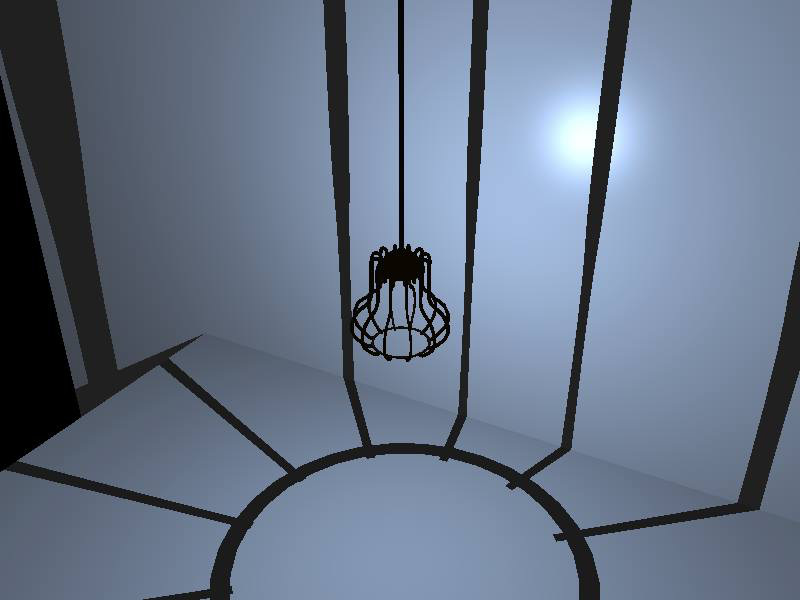
\includegraphics[width=5cm]{lampe_test1}
  \caption{Rendering af et 800x600 billede med en farvetemperatur på 15.000 kelvin samt synsvinklen V -0,5 og H 0,5.}
    \label{fig:lampe_test1}
\end{figure}

Vi vil nu teste om det er muligt at skifte farvetemperatur og synsvinkel. For at gøre dette ændres brugerinputtet:
\begin{lstlisting}
./trace model.ply -o  lamp.pnm -w 800 -h 600 -t 1200 -V 0.2
\end{lstlisting}

Farvetemperaturen er nu sat til 1200 kelvin og synsvinklen er sat til en vertikal vinkel på 0.2 radian. Det vi forventer er, at belysningen bliver orange og at billedet ses lige på med en negativ hældning på 0.2 radian. Renderingen ses på figur \ref{fig:lampe_test2}.

\begin{figure}[H]
  \centering
  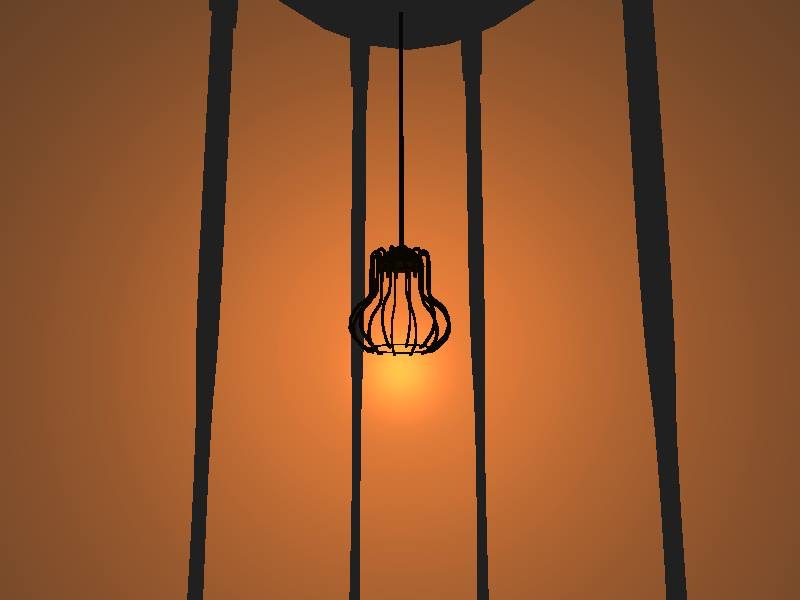
\includegraphics[width=5cm]{lampe_test2}
  \caption{Rendering af et 800x600 billede med en farvetemperatur på 1200 kelvin samt synsvinklen V 0,2}
    \label{fig:lampe_test2}
\end{figure}

Som der ses på billedet er belysningen orange som forventet og lampen er set lige på med en negativ vertikal hældning. Da testen gik som forventet er der nu verificeret, at det er muligt at ændre farvetemperatur og synsvinkel. Derudover ses det, at det er muligt for brugeren at indtaste en oplysning og en 3D-model og krav 1 er derfor verificeret.



\subsubsection{Test af optimering}

I følge krav 2 i afsnit, \ref{sec:teori} så skulle tiden det tog for at rendere et billede optimeres ved brug af KD-træer. Dette afsnit vil nu undersøge og KD-træer har formået at optimere renderingstiden. For at gøre dette køres programmet to gange med samme 3D-fil, og de to renderingstider sammenlignes. Figuren der blev renderet ses nedenfor:

\begin{figure}[H]
  \centering
  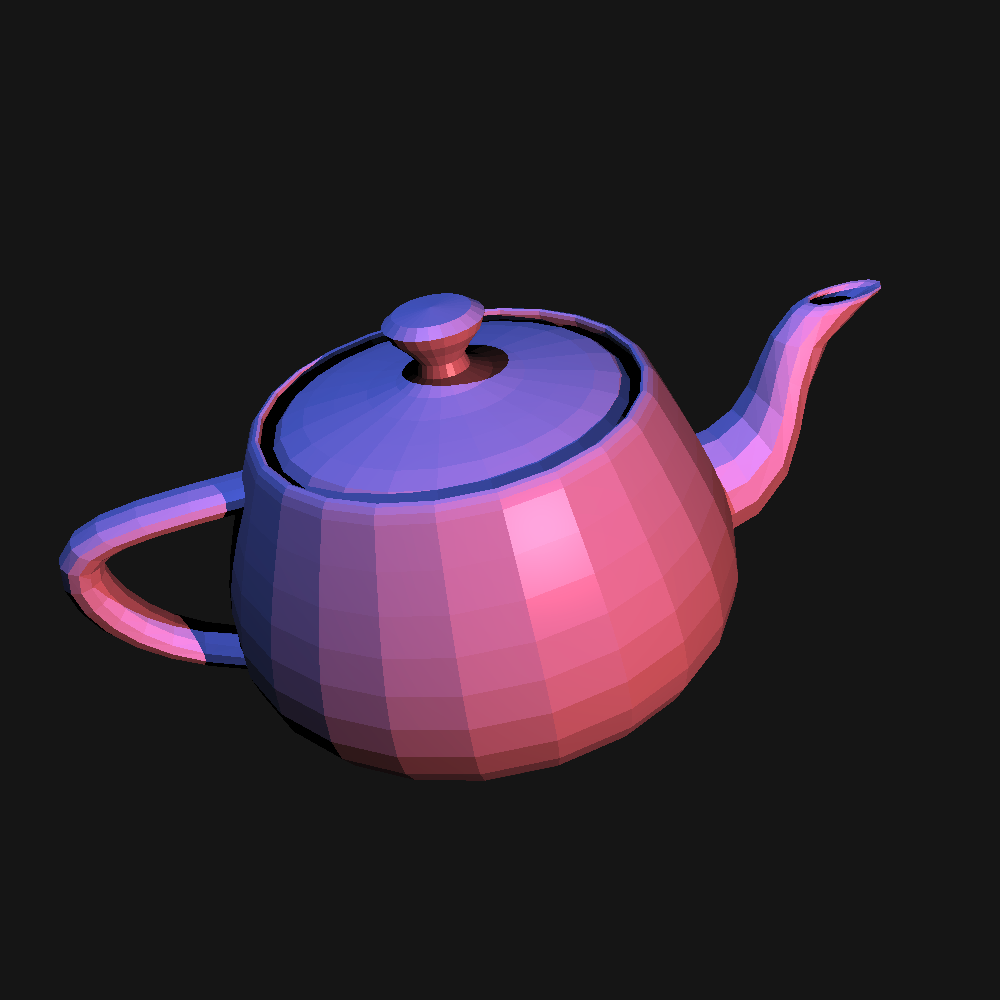
\includegraphics[width=5cm]{tekande}
  \caption{Rendering af en tekande.}
    \label{fig:tekande}
\end{figure}

Først køres programmet på den gamle algoritme:
\begin{lstlisting}
./trace teapot.old.ply
\end{lstlisting}
Terminaloutputtet er her illustreret i en listing:
\begin{lstlisting}
0.1%
0.2%
.
.
.
99.9%
100%
885s
\end{lstlisting}

Der ses altså at renderingstiden for figur \ref{fig:tekande} er på 885 sekunder med den gamle algoritme.

Programmet køres nu på det færdige program efter kd-træer er implementeret.
\begin{lstlisting}
./trace teapot.ply
\end{lstlisting}
Outputtet er:
\begin{lstlisting}
0.1%
0.2%
.
.
.
99.9%
100%
109s
\end{lstlisting}

Den nye renderings tid for figur \ref{fig:tekande} er på 109 sekunder efter optimeringen, det vil altså sige en forbedring på ca. 712\% og en faktisk stigning på 8.12 i forhold til den gamle algoritme. Der kan derfor udledes, at for figur \ref{fig:tekande} er det blevet over 8 gange så hurtigt at renderer figuren efter optimeringen. Krav 2 om optimering med KD-træer er derfor opfyldt.   

\subsubsection*{Opsummering}
Resultatet af programtestene var:

\begin{enumerate}
    \item Programmet kan rendere et billede ud fra følgende brugerinput: 3D-mode, opløsning, farvetemperatur og synsvinkel.
    \item Programmet er blevet optimeret ved brug af KD-træer
    \item Programmet kan gemme billedet.
\end{enumerate}

De tre programkrav i afsnit \ref{sec:teori} er derfor opfyldt.
